\documentclass[a4paper,11pt,twoside,openright]{book}
%% For screen reading please replace documentclass with:
%% \documentclass[a4paper,11pt]{report}

\usepackage{graphicx}
\usepackage{algorithmic}
\usepackage{algorithm}
\usepackage{listings}
\usepackage{booktabs}
\usepackage{amsmath}
\usepackage{setspace}
\usepackage{verbatim}
\usepackage[numbers]{natbib}
\usepackage[greek,english]{babel}
\usepackage[utf8x]{inputenc}
\usepackage{hyperref}
\usepackage{slantsc}
\usepackage[T1]{fontenc}

\hypersetup{
    bookmarks=true,            % show bookmarks bar?
    unicode=true,              % non-Latin characters in Acrobat’s bookmarks
    pdftoolbar=true,           % show Acrobat’s toolbar?
    pdfmenubar=true,           % show Acrobat’s menu?
    pdffitwindow=true,         % window fit to page when opened
    pdftitle={Master Thesis},  % title
    pdfborder={ 0 0 0 }        % uBorder tin links
}

\long\def\symbolfootnote[#1]#2  
    {\begingroup
    \def\thefootnote{\fnsymbol{footnote}}\footnote[#1]{#2}
    \endgroup}
\renewcommand{\baselinestretch}{1}\small\normalsize
\textwidth=390pt
\oddsidemargin = 50pt
\evensidemargin = 0pt

%% For screen reading please replace odd/even side margin with:
%% \oddsidemargin = 25pt
%% \evensidemargin = 25pt

\newcommand{\worksupportedby}{\symbolfootnote[0]{
Optionally: 
This work was partially supported by {\bf fill in sponsor name}
}}
\newcommand{\thesisdate}{July 2015}

\begin{document}
\lstset{language=C++}
\begin{titlepage}
\begin{center}

\LARGE \textbf{Thesis Title}\\[0.5cm]
\LARGE \textit{Christos Papoulas}\\[0.5cm]

\vfill

\normalsize{
Thesis submitted in partial fulfillment of the requirements for the\\[0.30cm]

\textit{Masters' of Science degree in Computer Science}}\\[0.30cm]

University of Crete\\
School of Sciences and Engineering\\
Computer Science Department\\
Knossou Av., P.O. Box 2208, Heraklion, GR-71409, Greece\\[0.5cm]

\vfill

\Large{Thesis Advisors: Prof. \emph{Kostas}, Dr. \emph{Magoutis}}\\[0.5cm]

\vfill

\end{center}

\worksupportedby{}
\end{titlepage}

\thispagestyle{empty}

\newcommand{\thesistitle}{Design and Implementation of a Social Networking Architecture for Cloud Deployment Specialists}
\newcommand{\owner}{Christos Papoulas}
\newcommand{\firstprof}{Manolis G.H. Katevenis}
\newcommand{\secondprof}{Kostas Magoutis}
\newcommand{\thirdprof}{Dimitris Plexousakis}
\newcommand{\chair}{Antonis Argyros}

\begin{titlepage}

\begin{center}
\textsc{University of Crete}\\
\textsc{Computer Science Department}\\
\vspace{0.4cm}
\noindent {\textbf{\thesistitle{}}}\\
\vspace{0.4cm}
\noindent Thesis submitted by\\
\textbf{\owner{}}\\
in partial fulfillment of the requirements for the\\
Masters' of Science degree in Computer Science\\
\vspace{0.4cm}
THESIS APPROVAL 

\vspace{0.4cm}

\begin{tabular}{rl}
\\
Author: & \underline{\phantom{123456789012345678901234567890123456789012}}\\
    & \owner{}\\
    \\
    \\
    \\
Committee approvals: & \underline{\phantom{123456789012345678901234567890123456789012}}\\
    & \firstprof{}\\
    & {\small Professor, Thesis Advisor}\\
    \vspace{0.2cm}
    \\
    \\
& \underline{\phantom{123456789012345678901234567890123456789012}}\\
    & \secondprof{}\\
    & {\small Assistant Professor, University of Ioannina, Thesis Co-advisor}\\
    \vspace{0.2cm}
    \\
    \\
& \underline{\phantom{123456789012345678901234567890123456789012}}\\
    & \thirdprof{}\\
    & {\small  Professor, Committee Member}\\
    \vspace{0.2cm}
    \\
    \\
\hspace{1.4ex}Departmental approval: & \underline{\phantom{123456789012345678901234567890123456789012}}\\
    & \chair{}\\
    & {\small  Professor, Director of Graduate Studies}\\
\end{tabular}
\\

\vfill
Heraklion, \thesisdate{}
\end{center}

\thispagestyle{empty}

\end{titlepage}

\thispagestyle{empty}
\begin{titlepage}
\begin{center}
{\bf\Large Abstract}\\
\end{center}

\indent In this work we propose a Social Network Platform, both front-end and back-end technology, for model-driven software design and deployment of applications in Multi-cloud environments. Nowadays, DevOps users wander around the web for automated tools like Chef supermarket, IBM bluemix and other deployment tools where almost manually configure and deploy their applications without any model-driven concept. The users can create their own Cloud Application Modeling and Execution
Language models or benefit from automatically generated models. We provide a Platform with an integrated community helping the DevOps users to deploy their applications. We incentivize user to stay inside the Platform instead of travel around the web for other Q\&A sites like StackOverflow to find their answers. The runtime executions of applications can be uploaded and analysed by the Platform presenting cost effectiveness analysis.


\vfill
\end{titlepage}


\thispagestyle{empty}
\selectlanguage{greek}
\begin{titlepage}
\begin{center}
{\bf\Large{Περίληψη}}\\
\end{center}

\indent  

Μια νέα τάση ανάμεσα στην ανάπτυξη και την λειτουργία των συστημάτων εφαρμογών που είναι γνωστή ως  \selectlanguage{english}DevOps\selectlanguage{greek} έχει γνωρίσει σημαντική ανάπτυξη τελευταία. Ένα τμήμα των μηχανικών \selectlanguage{english}DevOps\selectlanguage{greek}, οι οποίοι είναι ειδικοί στην προσαρμογή και εγκατάσταση των εφαρμογών σε περιβάλλοντα υπολογιστικού νέφους (επίσης γνωστοί ως \selectlanguage{english}cloud deployment specialists\selectlanguage{greek}), χρησιμοποιούν όλο και περισσότερο συγκεκριμένα εργαλεία για την εγκατάσταση των εφαρμογών τους όπως το \selectlanguage{english}Chef Supermarket\selectlanguage{greek} και το \selectlanguage{english}IBM Bluemix\selectlanguage{greek}.
Παρά την ύπαρξη αυτομάτων μηχανισμών, η κατάληξη σε καλή εγκατάσταση ακόμα απαιτεί συζήτηση με ειδικούς σε διαδικτυακά τεχνικά φόρουμ και κοινωνικά δίκτυα. 

Ανάμεσα στην κοινότητα των  \selectlanguage{english}DevOps\selectlanguage{greek}, η συζήτηση γύρω από την δομή των εφαρμογών και τα αποτελέσματα της εγκατάστασης σε υπολογιστικά νέφοι μπορεί να γίνει πιο εποικοδομητική γεφυρώνοντας τις τεχνολογίες των κοινωνικών δικτύων με την γνώση που υπάρχει στους χώρους δεδομένων που πηγάζουν από την παγκόσμια κοινότητα. Σε αυτήν την εργασία προτείνουμε μια πλατφόρμα κοινωνικού δικτύου (που παίρνει το όνομά της από το \selectlanguage{english}PaaSage EU project\selectlanguage{greek}) όπου οι ειδικοί στην εγκατάσταση σε περιβάλλοντα νέφους μπορούν να περιγράψουν τις εφαρμογές και τις απαιτήσεις τους ως μοντέλα εφαρμογών (χρησιμοποιώντας την \selectlanguage{english}Cloud Application Modeling and Execution Language\selectlanguage{greek} ή \selectlanguage{english}CAMEL\selectlanguage{greek}). Ακόμα μπορούν να συλλέξουν τα αποτελέσματα των εκτελέσεων των εφαρμογών σε πολλαπλά υπολογιστικά νέφη και να τα αποθηκεύσουν σε ένα χώρο δεδομένων που έχει δημιουργηθεί για αυτόν τον σκοπό. Τέλος, μπορούν να συζητήσουν με άλλους ειδικούς πάνω στα θέματα σχεδίασης και εγκατάστασης των εφαρμογών χρησιμοποιώντας αποτελέσματα εκτελέσεων.

Η υλοποίηση της πλατφόρμας κοινωνικής δικτύωσης του \selectlanguage{english}PaaSage\selectlanguage{greek} παρέχει στους χρήστες πληροφορίες που έχουν προέλθει από συλλογές εκτελέσεων κατανεμημένων εφαρμογών,  διευκολύνοντάς τους στην επιλογή της πλατφόρμας εγκατάστασης με βάση πληθώρα κριτηρίων (όπως η αποτελεσματικότητα κόστους). Η έρευνά μας εξερευνά και αξιολογεί διάφορες τεχνικές για την βελτίωση της κλιμακωσιμότητας της πλατφόρμας. Τέλος, για να κατευθύνουμε τους ειδικούς στην εγκατάσταση εφαρμογών στις βέλτιστες πιθανές απαντήσεις στης ερωτήσεις τους αξιοποιήσαμε εργαλεία κατηγοριοποίησης θεμάτων για να συσχετίσουμε τις ερωτήσεις των χρηστών με σχετικές ερωτήσεις και απαντήσεις (μερικές από τις οποίες μπορεί να περιλαμβάνουν αποτελέσματα από επερωτήσεις πάνω σε παλαιότερες εκτελέσεις εφαρμογών).


\vfill

\end{titlepage}

\selectlanguage{english}

\thispagestyle{empty}
\begin{titlepage}
{\bf\Large Acknowledgements}\\

Test acks \ldots

\vfill
\end{titlepage}

\pagenumbering{Roman}
\pagestyle{plain}
\tableofcontents
\listoffigures\listoftables
\pagenumbering{arabic}
\pagestyle{headings}
\chapter{Introduction}
In this work, the design and implementation of a social networking platform for designers of Multi-Cloud applications is presented. In this targeted social networking platform, DevOps engineers~\cite{loukides2012devops} and particularly cloud deployment specialists can benefit from other users' experience and answer design questions such as which is the most cost-effective deployment and which configuration best fits their needs. 

DevOps community consists of several types of specialists from both Development and Operations fields, such as programmers, testers, Quality Assurance staff~\cite{rossberg2014collaboration} from the first and system administrators from the second.  All the above professionals require different tools for various purposes like building applications, testing, deploying routines, configuration, automation of utilities, tracking and versioning in systems.  
Cloud Deployment Specialists are responsible for migration and configuration of hosted solutions for applications. Furthermore, they have deep industry knowledge about security, auto scaling, storage, load balancers, Content Delivery Networks~\cite{buyya2008content} and everything related to an application's secured hosting and scalability. The communication between these users is essential in order to exchange opinions and solutions on cloud deployment of applications. Having a repository, where they can find the configurations and the executions data of an application and point to those data is valuable since it can make their conversation specific and help them come to more concrete conclusions.

This social network targets the cloud deployment specialists and binds all social networking concepts such as personal messaging, groups, new feeds with concepts of application composition and deployment, integrating a repository of cloud applications and infrastructure description based on Cloud Application Modelling and Execution Language (CAMEL)~\cite{paasagedeliverable212}. 

This CAMEL repository brings to several benefits to the DevOps community.
Among the range of possible DevOps tasks, the Social Network focuses on selecting the most appropriate deployment
configuration for an application. This is especially challenging in a multi-cloud setting due to the
large diversity of deployment possibilities and tradeoffs. 

Currently DevOps users work with a small set of
well-understood deployment options, missing on opportunities for improving performance, reliability and/or
lower cost. Investigation of new options involves time consuming testing over new infrastructures. Discussing those topics with the community in online social or technical forums may provide insight over deployment options;
however, the answer to a hard question often needs to be backed by experimental data that is not readily
available. 

An integrated environment like our proposal, comes to solve the above issues by enriching user interactions with structured references to applications and their components, execution data, and mined knowledge from real deployments. Mined knowledge can be combined with user activity and profiles to provide personalized suggestions and hints.  An improved mode of user interaction is expected to result in stronger incentives for DevOps users to contribute information to the underlying repositories. Richer content should lead to better quality of mined knowledge, benefiting the DevOps community and providing further incentive for contributions.  The social networking platform designed to be closely integrated with a set of information repositories satisfying the following requirements: 
(R1) handle entire applications rather than just software components; (R2) abstract application structure through software modeling; (R3) capture and analyze application runtime performance. 

Altering the focus from the individual components of the applications to the whole applications and the analysis of its execution data, can provide answers to many interesting questions of the community and support discussions and arguments with hard data. 
These requirements can provide software developers with strong urge to contribute, leading to the sustainability and growth of information and derived knowledge in the repository.

This thesis is structured as follows: in the section ~\ref{sec:background} the background of application models and the CAMEL repository in the context of PaaSage EU project is presented. Chapter~\ref{sec:related} describes the previous work based on Caching architectures, other Social Networking Platforms and the Natural Language Processing. In the chapter~\ref{chap:implementation}, the system implementation of the Social Network is described and the chapter~\ref{chapt:evaluation} evaluates the implemented system. Finally, the present thesis concluded in chapter~\ref{sec:conclusions}.

\section{Background}
\label{sec:background}
This section presents an overview of the descriptions of the application models that are available on the Social Network Platform and a summary of the technologies that are used by the PaaSage in order to assist the cloud deployment specialists to deploy the aforementioned application models.

Application models inside social network platform are described in CAMEL. CAMEL integrates various domain-specific languages (DSLs).
DSLs provide a notation tailored towards an application domain and are based on the relevant concepts and features of that domain. As such, a DSL is a mean to describe and generate members of a family of programs in the domain. 
These DSLs cover a wealth of aspects of specification and execution of multi-cloud applications like CloudML, Scalability rules, WS Agreement, Saloon and Historical Execution Data. 

CloudML~\cite{FerryRossiniCMS13} is a recent approach that focuses on the provisioning and deployment of multi-cloud applications, is built upon MDE techniques and methods, and provides a models@run-time~\cite{models-runtime} environment for enacting the provisioning.  WS Agreement~\cite{andrieux2007web} is a Web Services protocol for establishing agreement between two parties, such as between a service provider and customer. Saloon ~\cite{quinton2013towards} is an approach that uses models to represent clouds variability, as well as ontologies to describe the heterogeneous aspect of the cloud ecosystem. The CAMEL model assembles all those DSLs as shown in figure~\ref{fig:dsls}.

CAMEL is using the Eclipse Modelling Framework (EMF)~\cite{steinberg2008emf} on top of the Connected Data Objects (CDO)~\cite{cdomodel}. Application Models are persisted on the CDO repository. EMF is used as a building tool for the application models. CAMEL model specification is written in XMI format (XML Metadata Interchange) which is a standard for exchanging metadata information via Extensible Markup Language (XML). Thus, XMI consists the main describing system of CAMEL and EMF provides tools that enable viewing and command-based or tree-based editing of the application models. 

\begin{figure}[h]
	\caption{CAMEL DSLs.}
	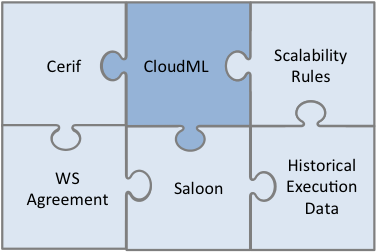
\includegraphics[width=0.6\textwidth,natwidth=200,natheight=150]{./fig/dsl.png}
	\centering
	\label{fig:dsls}
\end{figure}

The Social Network Platform that this thesis proposes is part of the PaaSage EU Project~\cite{paasage}.
The PaaSage perspective is to be a tool for a cloud deployment Specialist to leverage the complex task of deploying an application to the clouds. Usually, a cloud deployment specialist could easily learn the interface and features of one Cloud provider, but it would be very costly and time consuming to leverage the development to many providers. It is a real challenge to orchestrate the simultaneous deployment to many different Clouds at the same time. The main objective of PaaSage is to assist the developer to deal with difficult deployment scenarios through automatic cloud deployment. In order to satisfy this, several components are included to the PaaSage ecosystem. The Profiler components read the CAMEL models and convert them into a constraint programming model by defining the variables of the model, their domains, and the constraints that must be satisfied by the deployment. Also, the Profiler checks all constraints of the CAMEL model and sets the domains of the variables accordingly. The reasoning component analyses the model and finds how deployment candidates should be evaluated. Once a solution has been found, the reasoning component converts the model to Cloud Provider Specific Models (CPSM) for the providers involved in the proposed deployment. The adapter component takes the CPSMs, produces and validates a configuration plan, and sends this plan to the execution ware. The execution ware~\cite{baur2014towards} receives the deployment plan from the adapter and enacts the deployment of the application on the selected providers. Furthermore, the execution ware interacts with the Cloud providers, acquires the virtual machines, configures them and launches the user application on the set of virtual machines. Once the machines are running, the execution ware collects sensor data for the running application, triggering re-configurations if necessary.

The Social Network Platform brings to the DevOps users a friendly interface to browse, discover, view and discuss Application Models. Furthermore, it presents a way to deploy and run these Application Models, by using the previously mentioned components under the hood, and mines their execution history data.

The key contributions of this Social Network Platform(SNP) are the following:
\begin{itemize}
\item The SNP binds all the Social Networking aspects such as friends, new feeds, personal messages etc. with the engineering aspects of creating and deploying application models.
\item The SNP brings the execution histories of the CAMEL applications in the light, providing the end users the ability to browse, discus, point and find essential information needed for other applications.
\item The SNP uses the best known practices both for the front end viewing system and the back end technology.
\item The SNP runs on a horizontal scale architecture with memcached at the back end to reach near real time interaction. 
\end{itemize}



\section{Related Work}
This section describes related work for other professional networks and their caching architecture.

\subsection{Caching data}
Facebook, the largest social network, serves billions of requests per second using memcached~\cite{nishtala2013scaling}. In this magnitude of scale Facebook has several pools of memcached servers (regional pools) along the globe. A single request for a page can produce hundred of requests to the back-end system. Memcached used to store not only key-value from MySQL queries but also pre-computed results from sophisticated algorithms. 
In order to achieve a near real time communication experience to the end user, memcached server have to be efficient, reducing latency. 

The research question in such systems is when a particular key will be invalidated. This problem occurs according to ~\cite{nishtala2013scaling} in two cases: (1) \emph{stale sets} and (2) \emph{thundering herds}. A stale set occurs when a web server sets a value to the memcached that does not reflect the real value of the database. Thundering herds occur when a specific key has a heavy read and write activity in the same time. Stale sets resolved by a N-bit token, bound to specific key, sent from memcached to web server that want to update the key when cache miss occurs. If a delete request received then the request for updating this value from that client is rejected. The thundering herbs solved by configuring memcached servers return a N-bit token only once every ten seconds per key.

Linkedin, the largest professional network, stores hundreds of terabytes of data to Project Voldemord~\cite{sumbaly2012serving}, a key-value store, inspired by Amazon Dynamo~\cite{decandia2007dynamo}. Linkedin stores to Voldemort pre-computed offline data for example results of data mining applications such as features like ``People You May Know'' which running on hundreds of terabytes to make an estimation, using Hadoop as the computational component of those estimations. 
Voldemord compared with Dynamo has the same following requirements: (1) a simple \emph{get/put} application interface (2) A \emph{replication} factor, the number of replicas for each key-value tuble, implemented using vector clock (3) a \emph{required read} factor to succeed a get request, (4) a \emph{required write} factor to succeed a put request. 

\subsection{Professional Networks}

%During the last few years social networking has evolved into a fundamental daily activity for many individuals and a new frontier for business marketing. Besides “traditional” social networking, a recent trend is professional and domain-specific networking services focused on interactions and relationships of a business nature around a specific target domain. These online communities have the potential to become a platform for collective intelligence and open innovation~\cite{leimeister2010}, a medium for knowledge-centered collaboration~\cite{faraj2011}, and a trustworthy decision-support tool~\cite{bulmer2010}.
 
IT professionals use a variety of online sources as aids in their daily tasks. Developers typically prefer community-moderated forums over vendor-moderated sites. Social networks focusing on software technology in particular provide developers with the opportunity to leverage the knowledge and expertise of their peers.
 
One of the most popular such platforms is GitHub~\cite{github_url}, a collaborative revision control platform for developers launched in April 2008, and arguably the largest code-hosting site in the world. 
GitHub provides social networking functionality such as feeds, followers, wikis and a social network graph that captures how developers work on versions of their repositories, which version is newest, etc.
Gitter~\cite{gitter} is a related service that facilitates discussions between members of GitHub communities by providing a long-term chat integrated with code and issues.
Sourceforge~\cite{sourceforge} was the first code-hosting platform offered to open-source projects. It was launched in 1999 and offered IT professionals the ability to develop, download, review, and publish open-source software. Sourceforge is similar to GitHub in its support for social features.
Other similar code-hosting platforms are Google Code~\cite{googlecode} and Microsoft CodePlex~\cite{codeplex}.
None of those platforms collect, analyze, or use information from executions of application deployments to improve the level of technical discussion between users or abstract code structure through modelling or enhance user interactions through the use of analytics over application execution histories.

StackOverflow~\cite{stackoverflow} advances on earlier Q\&A sites in which users ask and answer questions. Users can vote up or down questions and answers and earn \emph{reputation points} and \emph{badges} in return for their active participation. 
Although StackOverflow and GitHub address different aspects of software development (StackOverflow is not a code-hosting platform) there is a synergy and correlation between the two~\cite{stackgit}. The proposed social network platform extends StackOverflow through the use of social networking features that enable users interested in reasoning about application deployments to use and share knowledge drawn from analyses of information repositories.
 
IBM's BlueMix~\cite{Bluemix-dev} is a development and support platform for communities of DevOps users wishing to compose distributed applications out of components drawn from libraries and deploy them at IBM-provided and supported cloud infrastructure.  BlueMix is a key component of IBM's DevOps best practices~\cite{ibm-devops} for achieving rapid prototyping, automated deployment, and continuous testing of software. BlueMix encourages its users to ask their questions to StackOverflow but also includes a community forum~\cite{Bluemix-dev} with rating of answers contributes to eventually building a basic knowledge base, similar to traditional approaches such as StackOverflow.  The proposed social network platform system differs from BlueMix in its support for expressing applications as models (CloudML, CAMEL) and its use of two information repositories, the PaaSage repository of models and execution histories and Chef supermarket, and the use of analytics over past executions to enable users to reason about application deployments. A common feature between the proposed social network platform and BlueMix is support for deployment of distributed applications. 

LinkedIn widely adopted across a range of professional communities due to its robust set of social features (and to some extent due to its use of extensive analytics over collected information~\cite{sumbaly2013big}), LinkedIn provides no specific support for software engineering activities and thus more closely resembles traditional social networking platforms such as Facebook.


The lack of Social Networking features of github came to fill the Geeklist platform~\cite{geeklist_url}, where developers and IT companies can discover and share the work they have done, connect with other companies with a social network manner or join development communities. Another code hosting platform is Snipplr ~\cite{Snipplr_url}, where developers can upload short code snippets and not full programs in order to keep all of their frequently used code in one place that's accessible from any computer and any user. Masterbranch~\cite{masterbranch_url} is a new under development platform that allows collating and sharing of projects within user profile. Profile works similarly to LinkedIn and has an incentivisation scheme called DevScore coupled with unlockable achievements in adds gamification element. Dzone~\cite{dzone_url} is essentially a link repository for developers allowing link sharing and incentivisation based around voting for popular links. The Code project~\cite{codeproject_url} website and forum allows code-specific discussion and shares relevant articles and news, contains blogs,  newsletter and has a questions and answers section.

The above systems can be further classified based on whether they use a repository to store software-related information (code, models, configuration, or execution histories) and whether this information is shared and raised through crowd sourcing~\cite{	howe2006rise}.  GitHub, GoogleCode, CodePlex, SourceForge, BlueMix, Chef Supermarket, and our platform store at least one type of software-related information and all systems but BlueMix are raising shared content in their software-related repositories via crowd sourcing. Our professional network is the only solution that analyzes information in its software-related repositories to assist users with suggestions and hints. 



\begin{table*}[h]

\begin{threeparttable}

\caption{Feature comparison.}
\label{tab:related}


\begin{tabular}{c|c|c|c|c|c|c|c|c|c|cc}

\cline{2-10}
  &  \multicolumn{4}{c|}{User Interaction} & \multicolumn{5}{c|}{Repository} &  &  \\ 
\cline{2-12} 
  &
   
  \begin{tabular}[c]{@{}c@{}}\rot{Social features \tnote{a}} \end{tabular} & 
  \begin{tabular}[c]{@{}c@{}}\rot{Groups} \end{tabular} &
  \begin{tabular}[c]{@{}c@{}}\rot{Q \& A} \end{tabular} &
  \begin{tabular}[c]{@{}c@{}}\rot{Personal  messaging} \end{tabular} & 
  \begin{tabular}[c]{@{}c@{}}\rot{Software code}\end{tabular} & 
  \begin{tabular}[c]{@{}c@{}}\rot{Software models}\end{tabular} & 
  \begin{tabular}[c]{@{}c@{}}\rot{Software config}\end{tabular} & 
  \begin{tabular}[c]{@{}c@{}}\rot{Execution histories}\end{tabular} & 
  \begin{tabular}[c]{@{}c@{}}\rot{Crowd sourced}\end{tabular} & 
  \multicolumn{1}{c|}{\begin{tabular}[c]{@{}c@{}}Repo\\ assisted\\ hints \tnote{b} \end{tabular}} & 
  \multicolumn{1}{c|}{\begin{tabular}[c]{@{}c@{}}Application\\ deployment\end{tabular}} \\ 
\hline

\multicolumn{1}{|c|}{GitHub} & \cmark & \xmark & \xmark & \xmark & \cmark & \xmark & \xmark & \xmark & \cmark & \multicolumn{1}{c|}{\xmark} & \multicolumn{1}{c|}{\xmark} \\
\hline
\multicolumn{1}{|c|}{Sourceforge} & \cmark & \xmark & \cmark & \cmark & \cmark & \xmark & \xmark & \xmark & \cmark & \multicolumn{1}{c|}{\xmark} & \multicolumn{1}{c|}{\xmark} \\
\hline
\multicolumn{1}{|c|}{GoogleCode} & \xmark & \xmark & \cmark & \xmark & \cmark & \xmark & \xmark & \xmark & \cmark & \multicolumn{1}{c|}{\xmark} & \multicolumn{1}{c|}{\xmark} \\
\hline
\multicolumn{1}{|c|}{CodePlex} & \cmark & \xmark & \cmark & \cmark & \cmark & \xmark & \xmark & \xmark & \cmark & \multicolumn{1}{c|}{\xmark} & \multicolumn{1}{c|}{\xmark} \\
\hline
\multicolumn{1}{|c|}{StackOverflow} & \xmark & \xmark & \cmark & \xmark & \xmark & \xmark & \xmark & \xmark & \xmark & \multicolumn{1}{c|}{\xmark} & \multicolumn{1}{c|}{\xmark} \\ 
\hline
\multicolumn{1}{|c|}{BlueMix} & \xmark & \xmark & \cmark & \xmark & \xmark & \xmark & \cmark & \xmark & \xmark & \multicolumn{1}{c|}{\xmark} & \multicolumn{1}{c|}{\cmark} \\ 
\hline
\multicolumn{1}{|c|}{Chef Supermarket} & \xmark & \xmark & \xmark & \xmark & \xmark & \xmark & \cmark & \xmark & \cmark & \multicolumn{1}{c|}{\xmark} & \multicolumn{1}{c|}{\xmark} \\ 
\hline
\multicolumn{1}{|c|}{LinkedIn} & \cmark & \cmark & \cmark & \cmark & \xmark & \xmark & \xmark & \xmark & \xmark & \multicolumn{1}{c|}{\xmark} & \multicolumn{1}{c|}{\xmark} \\ 
\hline
\multicolumn{1}{|c|}{geeklist} & \cmark & \cmark & \xmark & \xmark & \xmark & \xmark & \xmark & \xmark &  & \multicolumn{1}{c|}{ \xmark } & \multicolumn{1}{c|}{ \xmark } \\
\hline
\multicolumn{1}{|c|}{Snipplr} & \xmark & \xmark & \xmark & \xmark & \cmark & \xmark & \xmark & \xmark &  & \multicolumn{1}{c|}{\xmark} & \multicolumn{1}{c|}{\xmark} \\ 
\hline
\multicolumn{1}{|c|}{Masterbranch} & \xmark & \xmark & \xmark & \xmark & \cmark & \xmark & \xmark & \xmark &  & \multicolumn{1}{c|}{\xmark} & \multicolumn{1}{c|}{\xmark} \\ 
\hline
\multicolumn{1}{|c|}{Dzone} & \cmark & \xmark & \xmark & \xmark & \cmark & \xmark & \xmark & \xmark &  & \multicolumn{1}{c|}{ \xmark} & \multicolumn{1}{c|}{\xmark } \\ 
\hline
\multicolumn{1}{|c|}{codeproject} & \cmark & \xmark & \cmark & \xmark & \cmark & \xmark & \xmark & \xmark &  & \multicolumn{1}{c|}{\xmark} & \multicolumn{1}{c|}{\xmark} \\
\hline
\hline
\multicolumn{1}{|c|}{PaaSage SN} & \cmark & \cmark & \cmark & \cmark & \xmark & \cmark & \cmark & \cmark & \cmark & \multicolumn{1}{c|}{\cmark} & \multicolumn{1}{c|}{\cmark} \\ 
\hline

\end{tabular}

\begin{tablenotes}
      \small
       \item[a] Features: follow and news feed
      \item[b] User assistance based on data analysis of the repository
\end{tablenotes}
\end{threeparttable}
\end{table*}

\chapter{Management of ...}

General discussion \ldots

\section{AA}

\section{BB}

\section{CC}

\section{DD}

\chapter{Methodology}

General discussion \ldots

\section{AA}
\section{BB}
\section{CC}
\section{DD}
\section{EE}
\section{FF}

\chapter{Evaluation}
\label{chapt:evaluation}
This Chapter describes the evaluation of the scalability of the system architecture, the evaluation of the topic classification mechanism and the collaboration and contribution to user interface evaluation.  

\section{Scalability}
\label{sec:eval_scalability}
This Section describes the evaluation of the two different implementations of the system architecture. In the first architecture, more than one memcached instances at layer 2 were introduced, as Figure~\ref{fig:system_architecture} shows. In the second, more than one Social Network engines were introduced at layer 1.

In order to measure the response time (RT) the Apache JMeter application~\cite{jmeter_url} is used. The Apache JMeter is an open source benchmark designed to test functional behaviour and  measure performance, targeting web applications. Notably, the RT measured by JMeter may not be the real one, because the JMeter measures the elapsed time from just before sending the request to just after the last response from the server has been received. As a result, the time to render the web page to the client web browser and the execution time of JavaScript code is not measured. Because those two time intervals are client limited and depend on client performance and on which web browser is used, they are excluded from the following performance test benches. For the next experiments, a specific web page will be used. This page does not use any AJAX call, in order to not misguide the results. Therefore, the RT measures the time from just before JMeter sends the request to just after the last response is received. During this measured time interval, the Social Network engine performs the following actions:
\begin{enumerate}[I]
\item The Social Network engine sends a request to CDO Client for the application execution model.
\item The CDO Client forwards this request to CDO Server.
\item Afterwards CDO Server queries the mysql repository of application models and executions, and finally gets the executions results.
\item CDO Server forwards the results through the CDO Client to the Social Network Engine.
\item Finally, the Social Network engine sends queries to the Social Network DB in order to get all the necessary Social features for this application page
\end{enumerate}

The presented system architecture was deployed on Amazon EC2~\cite{amazon_url} and the system CPU Utilization and the response time of SNP is measured.

\subsection{Focusing on memcached}
\label{sec:eval_memcache}
By adding a Memcached node at the system architecture, the Social Network Engine first asks the Memcached node if it has the tuples that the SN Engine needs. So the steps(\emph{I} to \emph{V}), mentioned previously, are not necessary if the Memcached node has cached the values that the Social Network Engine needs. The loop through CDO CIient - CDO Server and the repositories is bypassed. 

\begin{table}[]
\centering
\caption{Number of Queries from Social Network and CDO server repository.}
\label{tab:num_of_queries}
\begin{tabular}{ll}
State        & \# of Queries \\
Fresh start  & 1938          \\
Fresh Query  & 15182         \\
Cached Query from CDO & 251           \\
Cached Query from Memcached & 147  
\end{tabular}
\end{table} 

For the following experiments all the Memcached nodes are warmed up and have already cached all the needed CDO and Social entities information. Furthermore the CDO server has been warmed up after a fresh restart. As the Table~\ref{tab:num_of_queries} shows,
the starting process of the CDO server produces 1938 queries to MySQL database. The \emph{fresh query} for an application model (both social information and executions) produces 15182 queries to MySQL database. The CDO server caches the results, so a second query for this application model produces 251 queries, most of which are the queries for the social information of the application. Introducing Memcached, if the request for the application model is cached, the queries to database are lowering to 147.  

\begin{figure}[h]
	\caption{The average response time for all configurations.}
	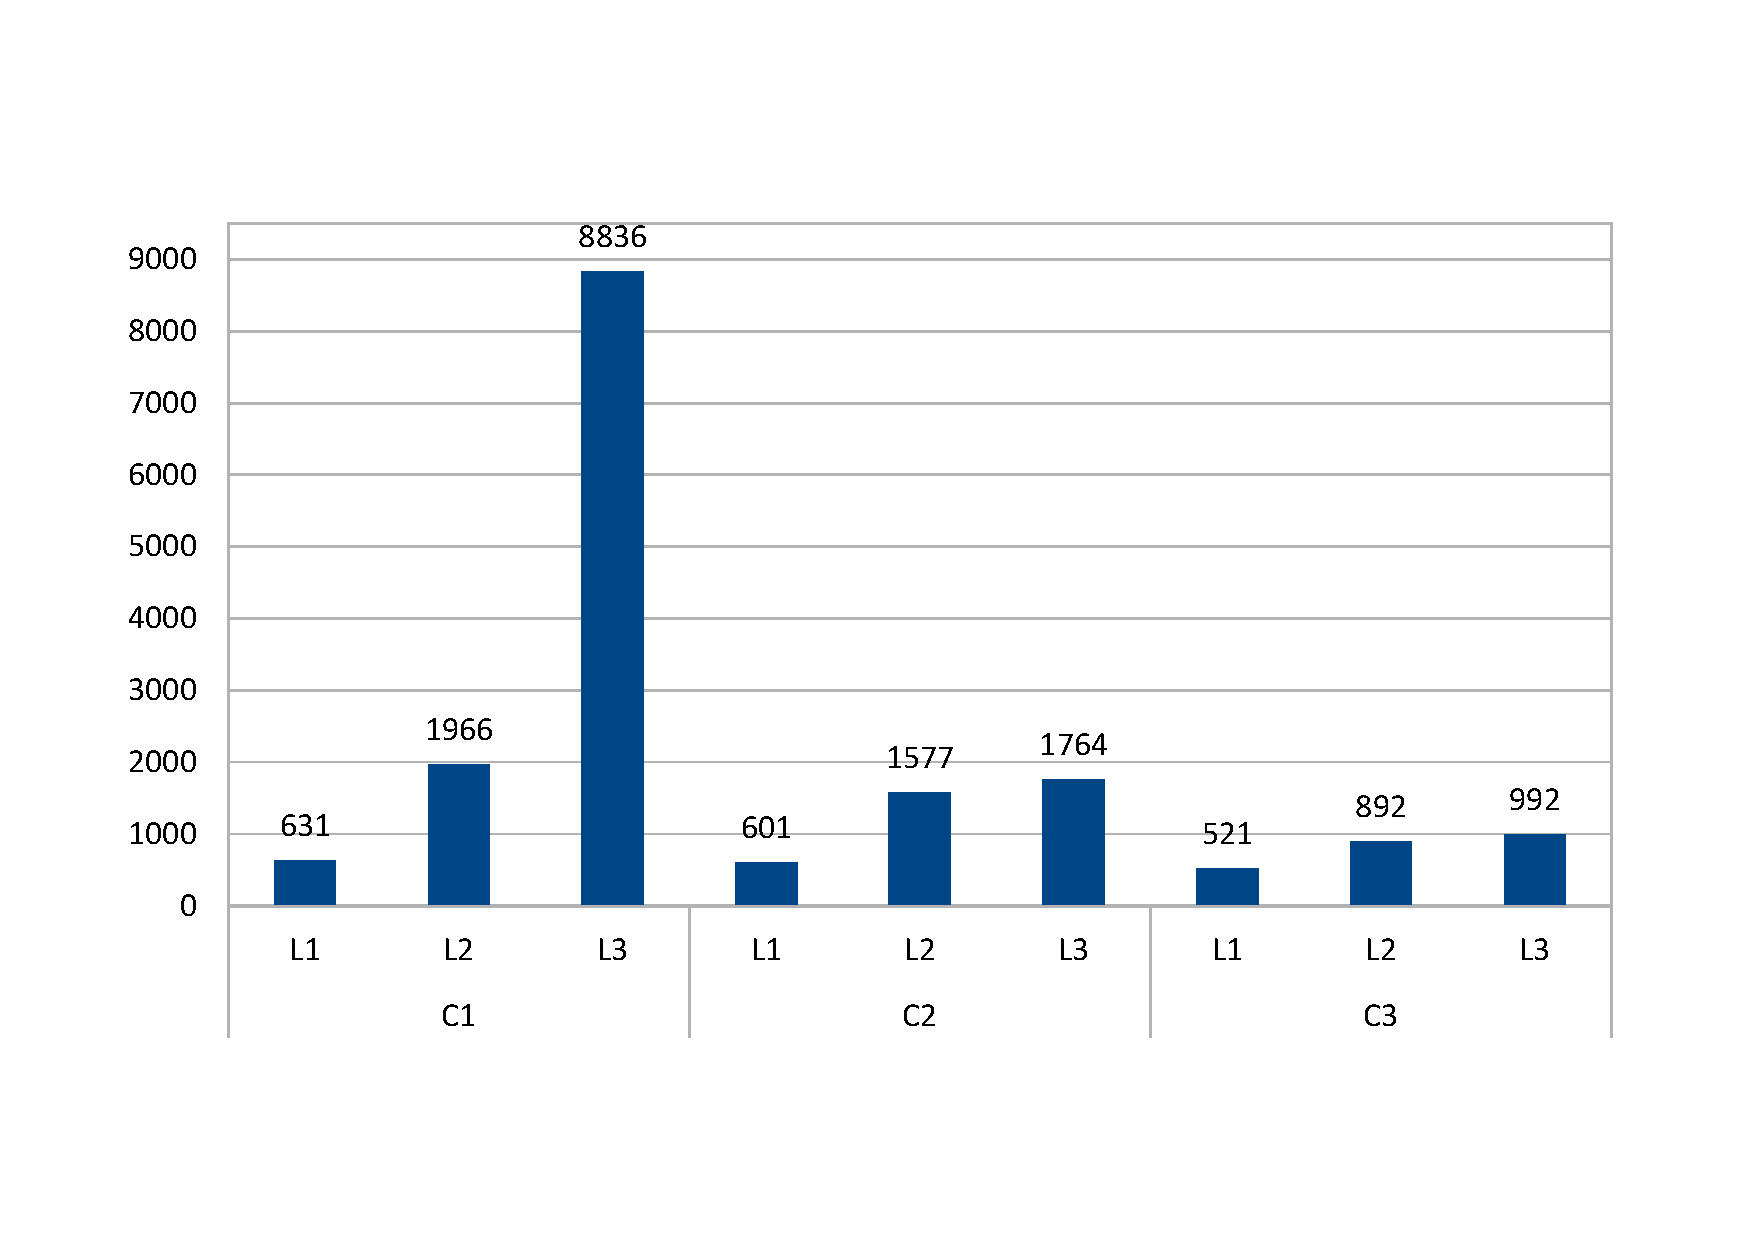
\includegraphics[width=0.9\textwidth,natwidth=200,natheight=150]{./fig/RTavg.pdf}
	\centering
	\label{fig:rtavg}
\end{figure}

The test performed with the following loads: (L1) ten users request \emph{two} applications, (L2) ten users request \emph{four} applications and (L3) ten users request \emph{eight} applications. All three Loads run consecutively one hundred times each. Those Loads request applications, which have ten execution rows pulled from the repository of applications models and executions, and about one hundred queries to the Social Network DB. In this experiment we kept the following components of the system constant: the Elgg front-end Apache2 server, the Social Network Database, and the CDO server - client communication but we increased the number of Memcached nodes.
The Figure~\ref{fig:rtavg} shows the  average response time (RT) in milliseconds with the following system configuration(C): (C1) no Memcached node , (C2) one Memcached node and (C3) two Memcached nodes have added to the system architecture.

As we going from C1 to C3 and specifically for L3, the RT is reduced by 80,4\% at C2 and by 88,78\% at C3. As the Figure~\ref{fig:rtavg} shows, at the first configuration C1, the L3 takes 8836 ms, an RT which is definitely prohibitive for web applications. Introducing more Memcached nodes at C2 and C3 the RT is decreased dramatically at 1764 ms at L2 and at 992 ms at L3. Going from C1 to C2, the 80,4\% reduction of RT is due to the introduction of Memcached node and bypassed the steps I - V. Going from C2 to C3, the 43,77\% reduction of RT. The reduction of RT is achieved by adding more Memcached nodes, which results to more CPU cores introduced to the architecture as described below.

\begin{figure}[h]
	\caption{The average CPU utilization for all components.}
	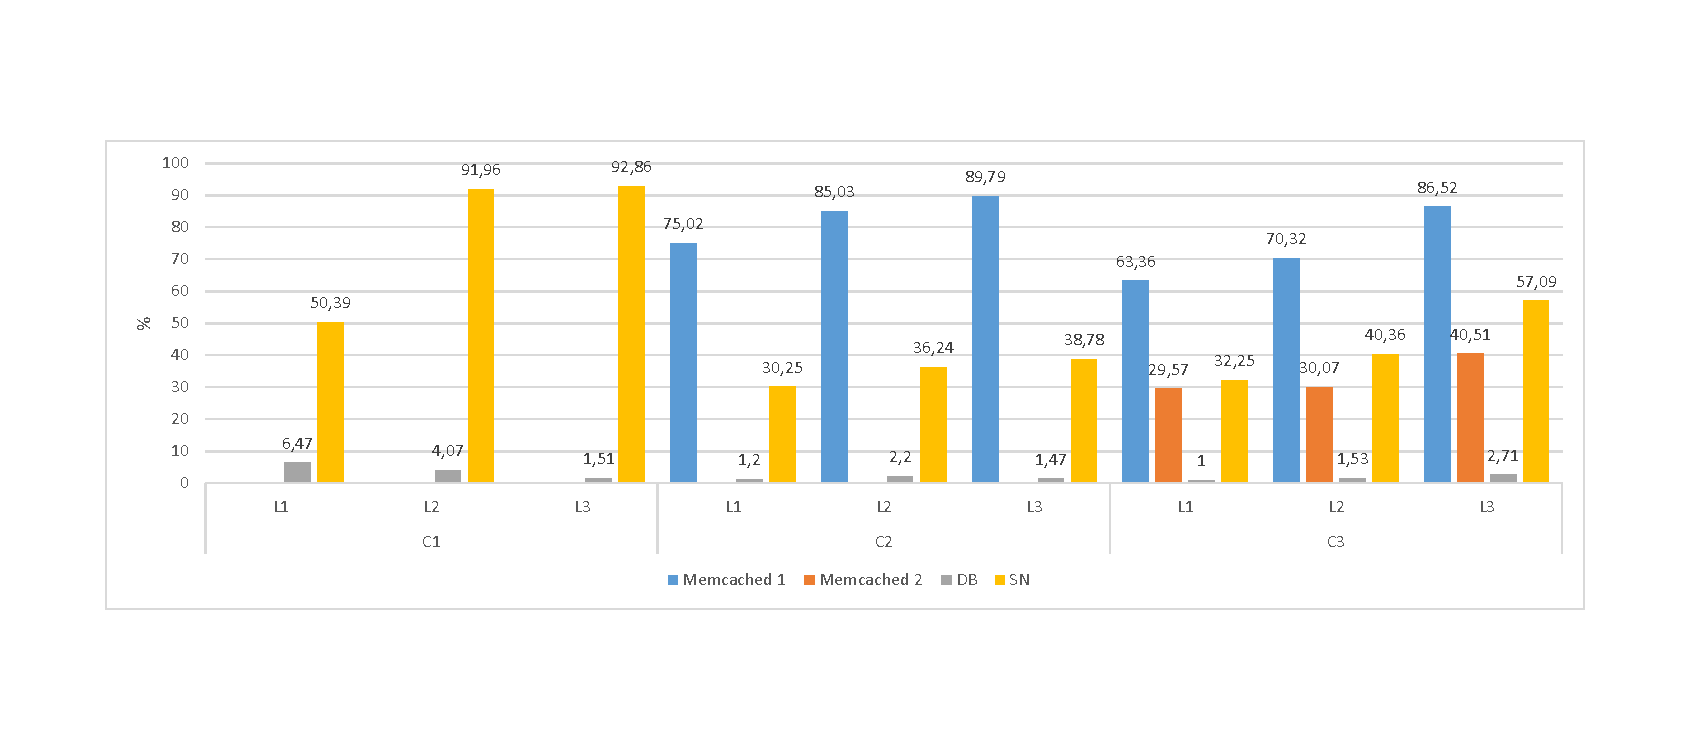
\includegraphics[width=1.1\textwidth,natwidth=200,natheight=250]{./fig/UsageAVG.pdf} 
	\centering
	\label{fig:cpuavg}
\end{figure}

The CPU utilization is measured using the sysstat tool~\cite{sysstat_url}. We measured the CPU utilization for all the VMs running the experiment. The information about the VM resources is listed in the Table~\ref{vms_resources}. The Social Network Engine and the CDO Client were running at t1.micro instance. The mysql (repositories) and the CDO Server were running at m1.xlarge. The average CPU utilization is shown in the Figure~\ref{fig:cpuavg}. At the simple configuration C1, even in small loads such as L1, the SN Engine reached 50,39\% CPU utilization. In the medium load L2 and big load L3 the SN Engine is kneeled down to 91,96\% and 92,86\%. This big consumption of CPU was due to all the initialization that Elgg Social Network Engine has to do for each request and due to CDO Server queries.

Moving from configuration C1 to C2, the CPU consumption went to Memcached node. Thus, the Social Network engine was de-congested and the RT improved. However, for the big load L3 the Memcached node reached 89,79\%. To solve Memcached CPU overhead, one more Memcached node was added at configuration C3. This second Memcached node shared the CPU overhead with the first Memcached node and the RT improved furthermore. 

For all three loads at C3, the first Memcached node had more CPU utilization from the second by an approximately factor of 2,2. This difference between the two Memcached nodes appeared due to the first node storing more popular key-value pairs than the other.

\begin{table}[]
\centering
\caption{VM resources. }
\label{vms_resources}
\begin{tabular}{|l|l|}
\hline
 Component &  VM type \\ \hline
 SN engine, CDO client &  t1.micro \\ \hline
 memcached &  t1.micro \\ \hline
 repositories, CDO Server &  m1.xlarge \\ \hline
 jmeter &  m1.large \\ \hline
\end{tabular}
\end{table}

\subsection{Focusing on the Elgg engine}

\begin{figure}[h]
	\caption{The Response time for two Social Network Engines.}
	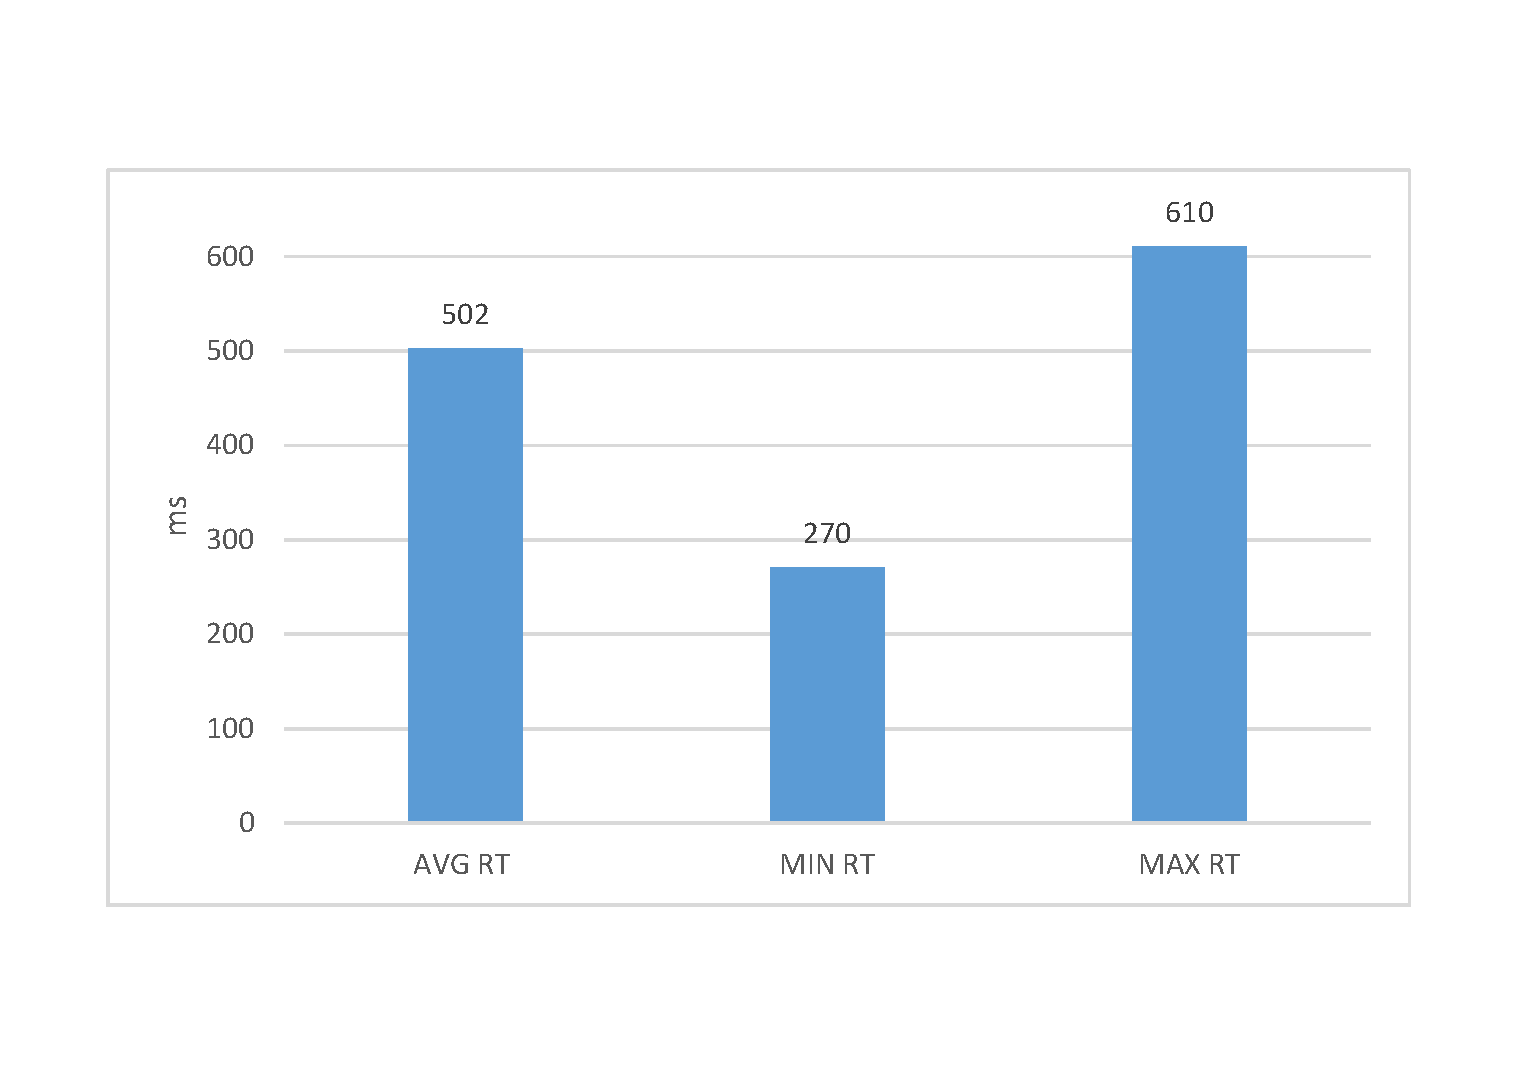
\includegraphics[width=0.8\textwidth,natwidth=200,natheight=150]{./fig/RT2SN.pdf}
	\centering
	\label{fig:rt2SN}
\end{figure}

\begin{figure}[h]
	\caption{The CPU utilization for two Social Network Engines.}
	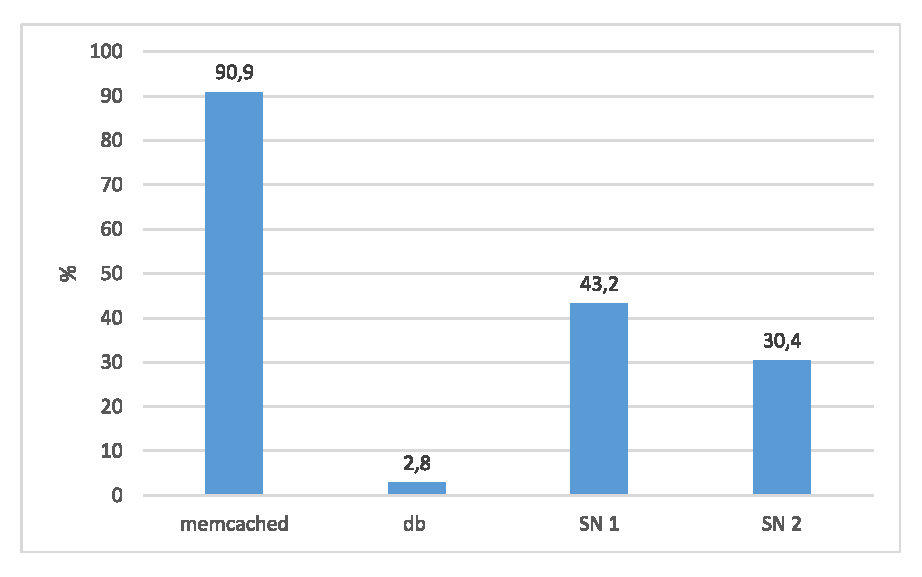
\includegraphics[width=0.8\textwidth,natwidth=200,natheight=150]{./fig/Usage2SN.pdf}
	\centering
	\label{fig:cpu2SNavg}
\end{figure}

This Section evaluates the horizontal scale of Social Network engine as described in~\ref{sec:engine_scale}. A memcached node was living between the Social Networking Engines and the back end system. The VM resources were kept the same as in the previous experiment and shown in the Table~\ref{vms_resources}. One more Social Networking Engine instance was added with the same type as former SN Engine. 

So, the system architecture now consists of two Social Networking Engines as front-end. At the back-end of the system we have: (1) one Memcached node and (2) the CDO client - server, the Social Network Database and the CDO repocitory. The two SN Engines are deployed to a dedicated VM each. Furthermore, each SN Engine has its own CDO client deployed with them. The Memcached node is deployed on its own VM and the CDO Server, the Social Network Database and the CDO repository are deployed on the same VM.

The Figure~\ref{fig:cpu2SNavg} shows the average CPU utilization for the Memcached, the MySql Database (db) and the two SN Engines (SN1, SN2). The load for this experiment is the same as the previous L3, which means we have ten users that request \emph{eight} applications for one hundred times consecutively. The first SN Engine has 43,2\% CPU usage and the second one has 12,8\% less. This difference is due to the first instance being deployed together with the NFS server and Apache Zookeeper on the same VM. 

With only one SN Engine the CPU Utilization was 57,09\% and now with two SN Engines the CPU Utilization is reduced to 43,2\%. This reduction is due to the requests being distributed to two instances instead of the only one instance. The CPU Utilization of the Memcached node increased, but this can be solved by introducing more Memcached nodes as the previous Section describes. Furthermore, we can introduce more SN Engines to support more heavy loads.

Since, the load from one SN Engine is now distributed to two SN Engines instances, the response time improved for the Load 3, as shown in the Figure~\ref{fig:rt2SN} compared to the previous test-bench. The best achieved RT of previous architecture was 992 ms and with this architecture it reduced to 502 ms.

We can combine the two architectures together, meaning that we have more than one SN Engine and more than one Memcached to support as many loads as we want.

\section{Topic classification}
\label{sec:nlp_evaluation}
This Section evaluates the topic classification tool as described in Section~\ref{sec:natural_implementation} for the first training set. This set had five different classes or, according to StackOverflow dialect, five tags, as described in~\ref{sec:natural_implementation} and shown in Table~\ref{table:nlp_eval}. For the testing set, thirty questions from StackOverflow were used per class. Those questions were different from the training set and had the highest activity during that specific time period. Each row at Table~\ref{table:nlp_eval} shows a class as classified by StackOverflow users, and each column shows how our classifier classifies the question. For example, twenty one questions about \emph{reliability} were classified correctly, but eight were wrongly classified as \emph{optimization} and one was wrongly classified as \emph{performance}. The misclassification however, was not an error of our classifier. The reason of these mistakes is that  some questions from the testing set were either wrongly classified by the StackOverflow users or had more than one tags. For example, one question that was wrongly classified as \emph{performance} instead of \emph{reliability} was: ``can somebody explain me how to handle errors. my code is: \ldots''. The above question is out of the scope of reliability and even though the user tagged it as a reliability question, it was downvoted and marked as ``very low quality'' from the StackOverflow community.

Another example showing that the classifier is not misclassifying, but the problem stands in the users' tagging, is the following question:
``I want to perform some data manipulation tasks and analysis in spark and want to \textbf{optimize} the run times. 
here is the problem: \ldots ''. 
This question was marked by the user with both scalability and optimization tags. Even though this question is retrieved with the scalability tag and in the Table~\ref{table:nlp_eval} it is shown as a wrong classification, after examining this question, one can realize that the \emph{scalability} tag was wrongly added by the user and only the \emph{optimization} tag should be placed.

This shows that our tool can further be used by StackOverflow to mark new questions that are wrongly tagged or misguided. There is a trend among StackOverflow users to add as many tags as they can in order to attract the attention of other users, increase the views of their question and finally get their answers.  

The true positive, which means a document is recognized in the correct class, according the Table~\ref{table:nlp_eval} is 85. The false positive, which means a document is not correctly recognized, of this topic evaluation is 65. According to those precision metrics the accuracy or sensitivity of our topic classifier for this specific experiment is 56,67\%.

\begin{table}[]
\centering
\caption{NLP Evaluation of Classification}
\label{table:nlp_eval}
\begin{tabular}{|l|c|c|c|c|c|}
\hline
class / class & \multicolumn{1}{l|}{reliability} & \multicolumn{1}{l|}{design} & \multicolumn{1}{l|}{optimization} & \multicolumn{1}{l|}{performance} & \multicolumn{1}{l|}{scalability} \\ \hline
reliability   & \textbf{21}                    & 0                           & 8                                 & 1                                & 0                                \\ \hline
design        & 2                                & \textbf{17}               & 6                                 & 3                                & 2                                \\ \hline
optimization  & 2                                & 3                           & \textbf{16}                     & 8 & 1                                \\ \hline
performance   & 1                                & 1                           & 11                                & \textbf{16}                     & 1                                \\ \hline
scalability   & 6                               & 3                           & 3                                 & 3                                & \textbf{15}                     \\ \hline
\end{tabular}
\end{table}

\section{Requirements and user interface}
\label{eval_ui}
The User Interface of social networking platform is designed through the iterative process of several expert-based evaluations being carried out in group sessions. To obtain additional feedback from non-experts, three additional user-based evaluation experiments were designed and carried out involving potential users and presented in~\cite{magoutis2015design}. 

The author collaborated in the expert-based evaluations sessions focusing on the platform user interface design. Furthermore, the contributions of the author, in the user interface evaluations, was to make the platform support them and also author took part in the third evaluation process.  

The first experiment, carried out by Flexiant Ltd. aimed at assessing the overall look and feel of the network, the navigation mechanisms, as well as the design of fundamental functionality.

The second evaluation experiment, carried out by HCI team, aimed to collect subjective results rather than performance metrics. It involved another set of 12 users who, after a brief introduction to the available facilities, were asked to use the interactive prototype~\cite{Virzi1996} using the free exploration method of the Thinking Aloud protocol~\cite{jordan1998introduction} and fill-in a questionnaire in order to rate and comment their experience. 

The third evaluation experiment involved 15 participants who were guided through the interactive prototype of the PaaSage social network using specific scenarios. They were interviewed on their requirements and feedback following a semi-structured interview approach [84]. The evaluation session was carried out via Skype. Participants were recruited through European companies and organizations associated with the PaaSage EU project~\cite{paasage}. They were either developers or operations staff, thus within the target user groups of the PaaSage social network. Participants were not users of the PaaSage platform; some however were familiar with the project’s goals and objectives. Before the experiment, each participant was requested to fill-in a background information form and was sent an informed consent form, explaining all the recording and anonymity-ensuring procedures. 

\begin{figure}[h]
	\caption{SNP features that were mostly liked by the users.}
	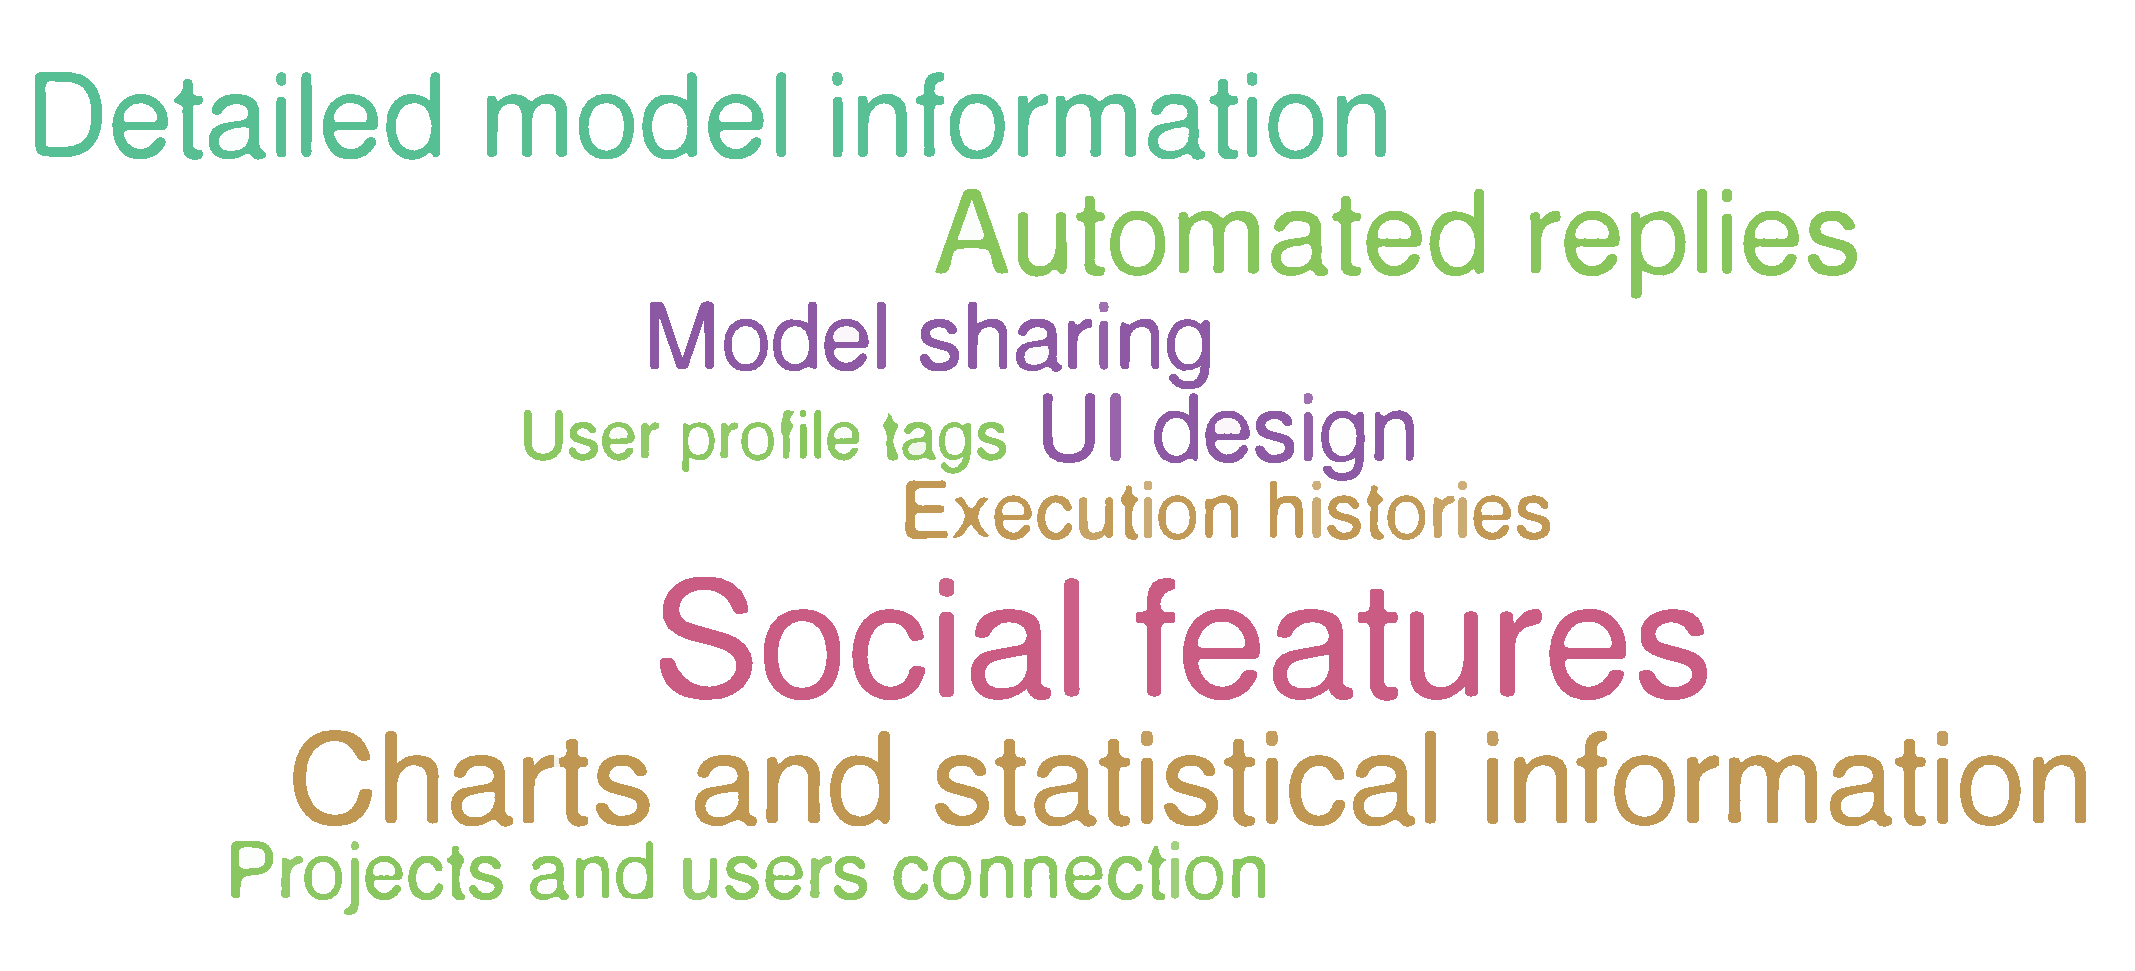
\includegraphics[width=1\textwidth,natwidth=200,natheight=150]{./fig/most-liked.pdf}
	\centering
	\label{fig:most-liked}
\end{figure}

Users, in the third experiment, were asked to identify up to three most-liked and three most-disliked features. Most-liked features presented in Figure~\ref{fig:most-liked} included: the employment of social features in a development environment; the use of charts and statistical information to represent data; the detailed model information that could be retrieved and the model execution histories; the automatically-generated hints provided by the network as replies in discussion topics; the concept of sharing one’s models; the overall UI design; the direct connection between projects and users, and the user profile tags that allowed them to find users that would be interesting to connect with.

Those evaluation experiments show that a platform that couples together the employment of social networking features in community-building activities with the DevOps demands about application deployment, the execution analysis, the automatically generated hints based on data analysis is a helpful tool that people would like to use.
\chapter{Comparison}

Compare your work \ldots

\section{AA}
\section{BB}

\chapter{Conclusions and Future Work}
In this thesis a scalable Social Network for DevOps users is presented. The scalining of the system presented at the front end layer by introducing more than one Social Networking Engine instances, or at the back end of the system by introducing more than one memcached nodes. The DevOps users of the Social Network can benefit from the \ldots
\bibliographystyle{IEEEtran}
\bibliography{references}

\end{document}
